\documentclass[a4paper,11pt]{jsarticle}


% 数式
\usepackage{amsmath,amsfonts}
\usepackage{bm}
% 画像
\usepackage[dvipdfmx]{graphicx}
% 図の先頭につく,fig.1とか図1とか(キャプション)のカスタマイズ
\usepackage{caption}
\captionsetup[figure]{labelformat=simple, labelsep=space, textfont=normalfont, labelfont=bf}
\renewcommand{\figurename}{Fig.}


\begin{document}

\title{進捗報告}
\author{渋谷享史}
\date{\today}
\maketitle
% 画像挿入
\begin{figure}[htbp]
  \vspace{5mm}
  \center
  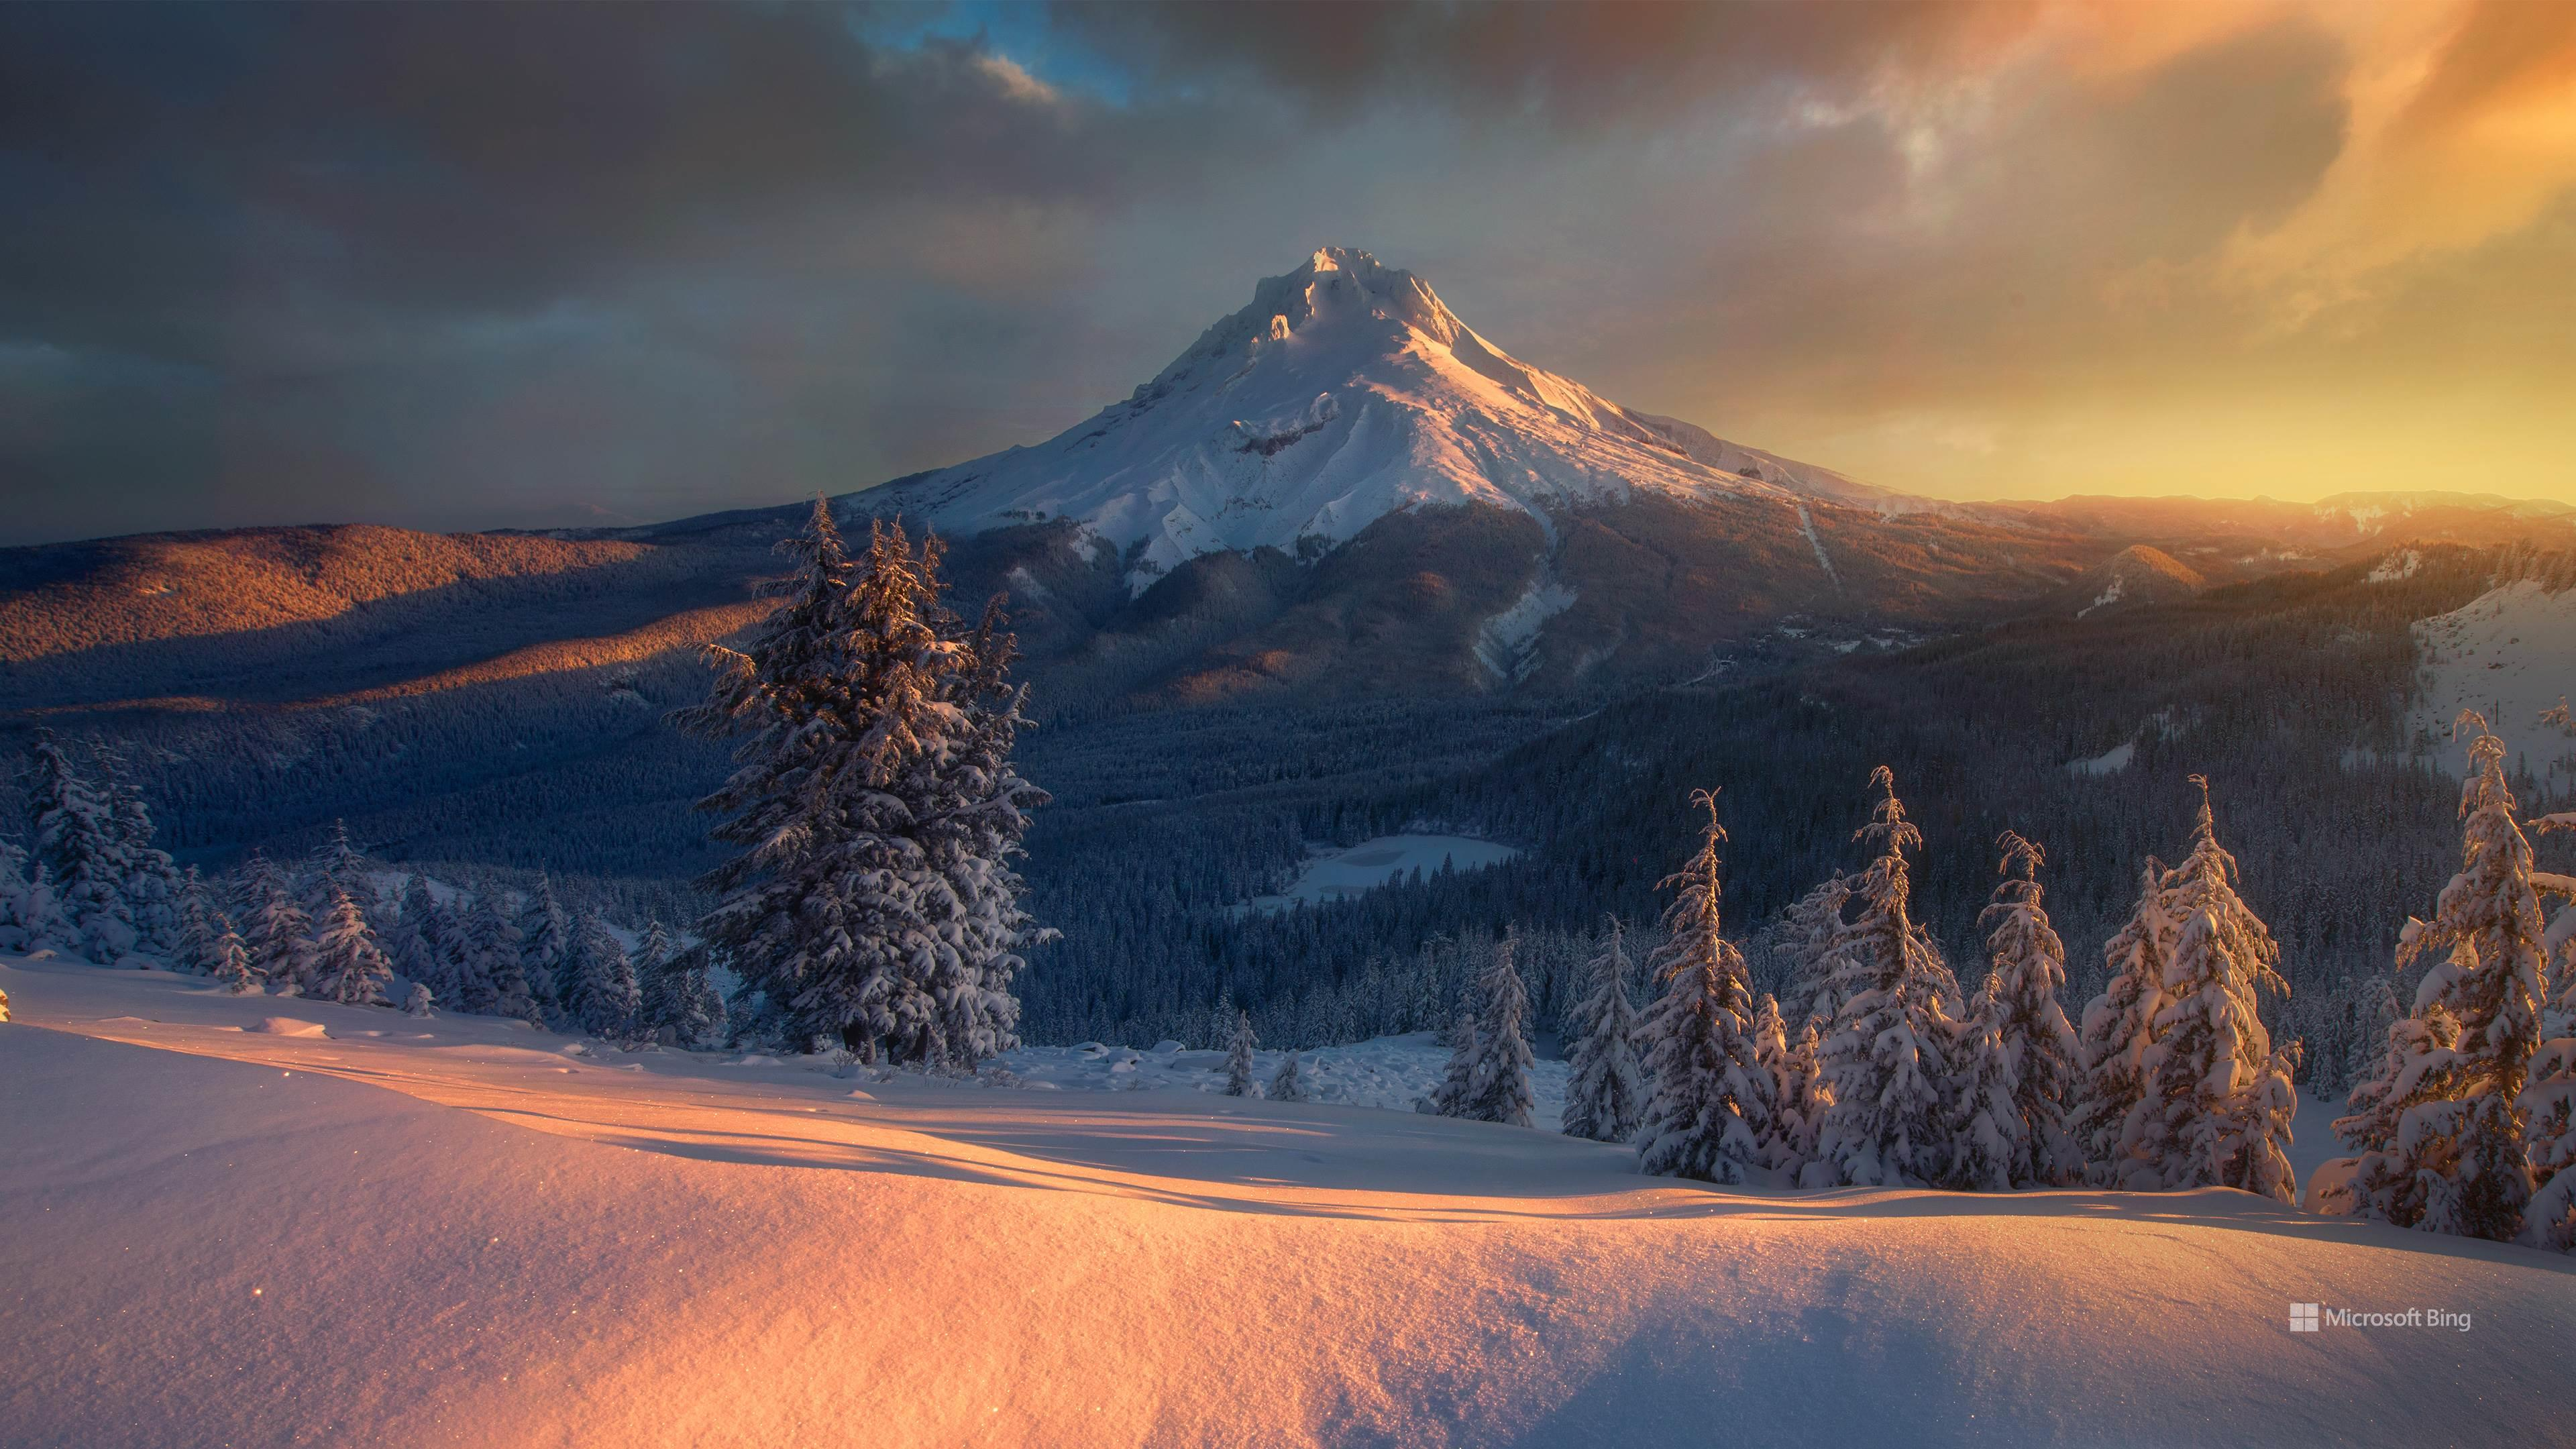
\includegraphics[width=100mm]{images/20240208.jpg}
  \caption{ブロック図}
  \label{block}
  \vspace{5mm}
\end{figure}

\end{document}
